\documentclass[tikz,border=0mm]{standalone}
\usetikzlibrary{arrows.meta,calc}
\newcommand{\tikzsetnextfilename}[1]{}

\definecolor{iconblue}{RGB}{70,140,255}
\definecolor{icongreen}{RGB}{78,158,114}
\definecolor{iconorange}{RGB}{225,139,63}

\tikzset{
  icon/.style={
    line width=1.2mm,
    line cap=round,
    line join=round
  },
  thinner/.style={line width=0.7mm},
  fine/.style={line width=0.4mm},
  node-blue/.style={
    circle,
    line width=0.55mm,
    fill=iconblue,
    draw=black,
    minimum size=6pt,
    inner sep=0pt
  },
  node-black/.style={
    circle,
    line width=0.55mm,
    fill=black,
    draw=black,
    minimum size=6pt,
    inner sep=0pt
  }
}

\newcommand{\cardframe}{%
  \useasboundingbox (-1,-1) rectangle (1,1);
  \draw[rounded corners=0.25cm] (-0.9,-0.9) rectangle (0.9,0.9);
}

\begin{document}

\tikzsetnextfilename{card-coxeterGroups}
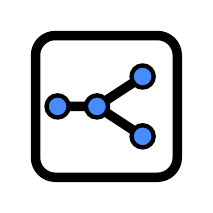
\begin{tikzpicture}[icon]
  \cardframe
  \coordinate (a) at (-0.62,0);
  \coordinate (b) at (-0.12,0);
  \coordinate (c) at (0.46,0.38);
  \coordinate (d) at (0.46,-0.38);
  \draw (a) -- (b) -- (c);
  \draw (b) -- (d);
  \foreach \p in {a,b,c,d} {
    \node[node-blue, minimum size=8pt] at (\p) {};
  }
\end{tikzpicture}

\tikzsetnextfilename{card-ehrhart}
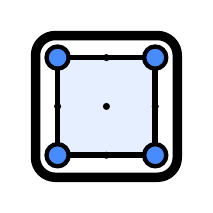
\begin{tikzpicture}[icon]
  \cardframe
  \fill[iconblue!14, draw=black, line width=0.7mm]
    (-0.62,-0.62) rectangle (0.62,0.62);
  \foreach \x in {-0.62,0,0.62} {
    \foreach \y in {-0.62,0,0.62} {
      \fill[black] (\x,\y) circle (0.045);
    }
  }
  \foreach \p in {(-0.62,-0.62),(-0.62,0.62),(0.62,-0.62),(0.62,0.62)} {
    \node[node-blue, minimum size=8pt] at \p {};
  }
\end{tikzpicture}

\tikzsetnextfilename{card-quasiSymmetricFunctions}
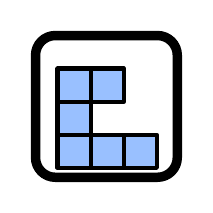
\begin{tikzpicture}[icon]
  \cardframe
  \begin{scope}[shift={(-0.62,0.48)}, scale=0.42]
    \foreach \x/\y/\w in {0/0/2,0/-1/1,0/-2/3} {
      \foreach \i in {0,...,\w} {
        \ifnum\i<\w
          \filldraw[fill=iconblue!55, draw=black, line width=0.55mm]
            (\i,\y) rectangle ++(1,-1);
        \fi
      }
    }
  \end{scope}
\end{tikzpicture}

\tikzsetnextfilename{card-slideM}
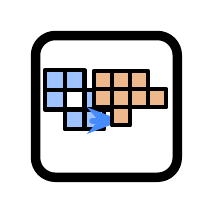
\begin{tikzpicture}[icon]
  \cardframe
  \begin{scope}[shift={(-0.78,0.46)}, scale=0.25]
    \foreach \x/\y in {0/0,1/0,0/-1,2/-1,3/-1,1/-2,2/-2} {
      \filldraw[fill=iconblue!52, draw=black, line width=0.55mm]
        (\x,\y) rectangle ++(1,-1);
    }
  \end{scope}
  \draw[iconblue, ->, >=Stealth, line width=0.75mm]
    (-0.18,-0.18) -- (0.2,-0.18);
  \begin{scope}[shift={(-0.16,0.45)}, scale=0.23]
    \foreach \x/\y in {0/0,1/0,2/0,0/-1,1/-1,2/-1,3/-1,1/-2} {
      \filldraw[fill=iconorange!60, draw=black, line width=0.55mm]
        (\x,\y) rectangle ++(1,-1);
    }
  \end{scope}
\end{tikzpicture}

\tikzsetnextfilename{card-totalPositivity}
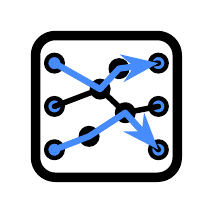
\begin{tikzpicture}[icon]
  \cardframe
  \foreach \y in {-0.55,0,0.55} {
    \node[node-blue] at (-0.66,\y) {};
    \node[node-blue] at (0.66,\y) {};
  }
  \foreach \x/\y in {-0.22/-0.38,-0.08/0.22,0.24/-0.08,0.16/0.48} {
    \node[node-black] at (\x,\y) {};
  }
  \draw[thinner] (-0.66,-0.55) -- (-0.22,-0.38) -- (0.24,-0.08) -- (0.66,-0.55);
  \draw[thinner] (-0.66,0) -- (-0.08,0.22) -- (0.24,-0.08) -- (0.66,0);
  \draw[thinner] (-0.66,0.55) -- (-0.08,0.22) -- (0.16,0.48) -- (0.66,0.55);
  \draw[iconblue, ->, >=Stealth, line width=0.8mm]
    (-0.66,-0.55) -- (-0.22,-0.38) -- (0.24,-0.08) -- (0.66,-0.55);
  \draw[iconblue, ->, >=Stealth, line width=0.8mm]
    (-0.66,0.55) -- (-0.08,0.22) -- (0.16,0.48) -- (0.66,0.55);
\end{tikzpicture}

\tikzsetnextfilename{card-spechtModules}

\begin{tikzpicture}[icon]
  \cardframe
  \begin{scope}[shift={(-0.66,0.46)}, scale=0.29]
    \filldraw[fill=iconblue!55, draw=black, line width=0.55mm]
      (0,0) rectangle ++(1,-1);
    \filldraw[fill=iconblue!30, draw=black, line width=0.55mm]
      (1,0) rectangle ++(1,-1);
    \filldraw[fill=iconorange!60, draw=black, line width=0.55mm]
      (0,-1) rectangle ++(1,-1);
    \draw[iconorange, line width=0.8mm] (0.5,0.18) -- (0.5,-2.18);
  \end{scope}
  \draw[black, fine, ->, >=Stealth] (-0.12,0.1) -- (0.12,0.1);
  \draw[black, fine] (-0.08,-0.25) -- (0.08,-0.25);
  \begin{scope}[shift={(0.22,0.46)}, scale=0.29]
    \filldraw[fill=iconorange!60, draw=black, line width=0.55mm]
      (0,0) rectangle ++(1,-1);
    \filldraw[fill=iconblue!30, draw=black, line width=0.55mm]
      (1,0) rectangle ++(1,-1);
    \filldraw[fill=iconblue!55, draw=black, line width=0.55mm]
      (0,-1) rectangle ++(1,-1);
    \draw[iconorange, line width=0.8mm] (0.5,0.18) -- (0.5,-2.18);
  \end{scope}
  \draw[iconblue, line width=0.85mm, rounded corners=0.05cm]
    (-0.58,-0.5) -- (-0.18,-0.68) -- (0.34,-0.68) -- (0.62,-0.5);
\end{tikzpicture}

\tikzsetnextfilename{card-zeroHeckeAlgebra}
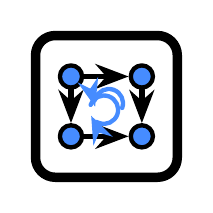
\begin{tikzpicture}[icon]
  \cardframe
  \node[node-blue, minimum size=8pt] (a) at (-0.45,0.38) {};
  \node[node-blue, minimum size=8pt] (b) at (0.45,0.38) {};
  \node[node-blue, minimum size=8pt] (c) at (-0.45,-0.38) {};
  \node[node-blue, minimum size=8pt] (d) at (0.45,-0.38) {};
  \draw[black, thinner, ->, >=Stealth] (a) -- (b);
  \draw[black, thinner, ->, >=Stealth] (c) -- (d);
  \draw[black, thinner, ->, >=Stealth] (a) -- (c);
  \draw[black, thinner, ->, >=Stealth] (b) -- (d);
  \draw[iconblue, line width=0.55mm, ->, >=Stealth]
    (-0.2,0.02) arc (160:-155:0.18);
  \draw[iconblue, line width=0.55mm, ->, >=Stealth]
    (0.2,-0.02) arc (-20:195:0.18);
\end{tikzpicture}

\tikzsetnextfilename{card-symmetricFunctions}

\begin{tikzpicture}[icon]
  \cardframe
  \begin{scope}[shift={(-0.58,0.56)}, scale=0.43]
    \foreach \x/\y in {0/0,1/0,2/0,0/-1,1/-1,0/-2} {
      \filldraw[fill=iconblue!50, draw=black, line width=0.55mm]
        (\x,\y) rectangle ++(1,-1);
    }
  \end{scope}
\end{tikzpicture}

\tikzsetnextfilename{card-nonComFunctions}
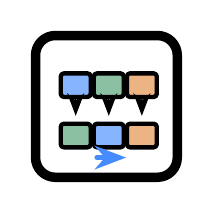
\begin{tikzpicture}[icon]
  \cardframe
  \foreach \x/\y/\c in {-0.58/0.42/iconblue,-0.16/0.42/icongreen,0.26/0.42/iconorange} {
    \filldraw[fill=\c!65, draw=black, line width=0.55mm, rounded corners=0.04cm]
      (\x,\y) rectangle ++(0.38,-0.3);
  }
  \foreach \x/\y/\c in {-0.58/-0.22/icongreen,-0.16/-0.22/iconblue,0.26/-0.22/iconorange} {
    \filldraw[fill=\c!65, draw=black, line width=0.55mm, rounded corners=0.04cm]
      (\x,\y) rectangle ++(0.38,-0.3);
  }
  \draw[black, fine, ->, >=Stealth] (-0.39,0.08) -- (-0.39,-0.12);
  \draw[black, fine, ->, >=Stealth] (0.03,0.08) -- (0.03,-0.12);
  \draw[black, fine, ->, >=Stealth] (0.45,0.08) -- (0.45,-0.12);
  \draw[iconblue, line width=0.65mm, ->, >=Stealth]
    (-0.12,-0.65) -- (0.25,-0.65);
\end{tikzpicture}

\tikzsetnextfilename{card-wordList}

\begin{tikzpicture}[icon]
  \cardframe
  \filldraw[fill=iconblue!18, draw=black, line width=0.6mm,
    rounded corners=0.06cm] (-0.55,-0.62) rectangle (0.48,0.62);
  \draw[black, thinner] (-0.34,0.62) -- (-0.34,-0.62);
  \foreach \y in {0.34,0.12,-0.10,-0.32} {
    \draw[black, line width=0.45mm] (-0.18,\y) -- (0.28,\y);
    \fill[iconorange] (-0.33,\y) circle (0.035);
  }
  \draw[icongreen, line width=0.8mm] (0.22,-0.38) circle (0.16);
  \draw[icongreen, line width=0.8mm] (0.33,-0.49) -- (0.56,-0.72);
\end{tikzpicture}

\tikzsetnextfilename{card-hivePolytopes}
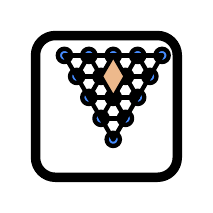
\begin{tikzpicture}[icon]
  \cardframe
  \begin{scope}[scale=0.31, shift={(-1.72,-1.35)}]
    \foreach \i in {0,...,4} {
      \foreach \j in {0,...,\i} {
        \coordinate (p\i\j) at ({\j+0.5*(4-\i)},{0.86*\i});
        \node[node-blue, minimum size=4.8pt] at (p\i\j) {};
      }
    }
    \foreach \i in {0,...,3} {
      \pgfmathtruncatemacro{\next}{\i+1}
      \foreach \j in {0,...,\i} {
        \draw[black, line width=0.55mm] (p\i\j) -- (p\next\j);
        \draw[black, line width=0.55mm]
          (p\i\j) -- (p\next\the\numexpr\j+1\relax);
      }
    }
    \foreach \i in {1,...,4} {
      \pgfmathtruncatemacro{\last}{\i-1}
      \foreach \j in {0,...,\last} {
        \draw[black, line width=0.55mm]
          (p\i\j) -- (p\i\the\numexpr\j+1\relax);
      }
    }
    \filldraw[fill=iconorange!60, draw=black, line width=0.5mm]
      (p21) -- (p31) -- (p42) -- (p32) -- cycle;
  \end{scope}
\end{tikzpicture}

\end{document}
